\chapter{Analiza wymagań}
% TO DO: dodać jakieś zagajenie

Analiza wymagań to kluczowy etap procesu tworzenia oprogramowania, który ma na celu zrozumienie potrzeb użytkowników oraz specyfikacji systemu. W przypadku projektowania aplikacji typu Elektroniczne Biuro Obsługi Klienta (eBOK) dla wspólnoty mieszkaniowej, istotne jest zidentyfikowanie wszystkich funkcjonalności, które będą odpowiadały zarówno mieszkańcom, jak i administratorom. Poprawna analiza wymagań pozwala na stworzenie systemu, który nie tylko spełnia potrzeby użytkowników, ale także jest skalowalny, bezpieczny i łatwy w utrzymaniu.

W niniejszym rozdziale zostaną omówione zarówno funkcjonalne, jak i niefunkcjonalne wymagania systemu, uwzględniając różnorodne potrzeby użytkowników. Przeanalizowane zostaną także kluczowe aspekty, takie jak bezpieczeństwo, wydajność, intuicyjność interfejsu, a także integracja z innymi systemami. Wymagania te będą stanowiły podstawę do zaprojektowania architektury systemu oraz jego implementacji.

\section{Zarys architektury systemu}
% TO DO: przedstawić (na diagramach poglądowych), jak ma wyglądać architektura systemu (z jakich komponentów będzie się ona składać, kto z niej będzie korzystać, jakie interfejsy będzie udostępniać). Może z tego będzie trzeba zrobić osobny rozdział.

Zarys architektury systemu jest kluczowym krokiem w projektowaniu oprogramowania, który pozwala na stworzenie efektywnego i funkcjonalnego rozwiązania. W przypadku aplikacji Elektronicznego Biura Obsługi Klienta (eBOK) dla wspólnoty mieszkaniowej, architektura musi uwzględniać zarówno potrzeby użytkowników, jak i wymagania techniczne. W tym rozdziale przedstawione zostaną główne komponenty systemu oraz ich wzajemne interakcje, na podstawie przedstawionego schematu.

\subsection{Komponenty systemu}

Architektura systemu eBOK składa się z kilku kluczowych komponentów, które współpracują ze sobą, aby zapewnić pełną funkcjonalność aplikacji. Do głównych komponentów należą:

\begin{itemize} 

	\item \textbf{Frontend} - Interfejs użytkownika aplikacji, zrealizowany w technologii Next.js, pisany w TypeScript. Frontend obsługuje interakcje użytkowników (mieszkańców oraz administratorów) oraz prezentuje dane w odpowiednim formacie. Komunikacja z backendem odbywa się za pośrednictwem bezpiecznego protokołu HTTPS, a dane są szyfrowane, przy pomocy protokołu TLS.

	\item \textbf{Backend} - Serwer aplikacji oparty na Spring Boot, działający w kontenerze Docker, odpowiedzialny za logikę biznesową oraz zarządzanie danymi. Backend zapewnia funkcje takie jak autoryzacja użytkowników (przez OAuth 2.0), obsługa zgłoszeń mieszkańców, zarządzanie płatnościami i komunikacja z zewnętrznymi systemami.

	\item \textbf{Warstwa logiki biznesowej} - Kluczowa część backendu odpowiedzialna za implementację reguł biznesowych, które obsługują funkcjonalności aplikacji, takie jak przetwarzanie zgłoszeń czy zarządzanie danymi użytkowników.

	\item \textbf{Warstwa dostępu do danych} - Odpowiada za komunikację z bazą danych PostgreSQL, przechowującą informacje dotyczące użytkowników, zgłoszeń, płatności i innych istotnych danych. Ta warstwa zapewnia trwałość i integralność danych w systemie.

	\item \textbf{Baza danych} - System PostgreSQL, działający w kontenerze Docker, przechowujący wszystkie kluczowe dane aplikacji. Dzięki konteneryzacji możliwe jest łatwe skalowanie i zarządzanie bazą danych w środowisku produkcyjnym.

	\item \textbf{Serwer OAuth 2.0} - Serwer autoryzacji, który zapewnia bezpieczeństwo dostępu do zasobów systemu przez użytkowników. OAuth 2.0 umożliwia zarządzanie autoryzacją dostępu, co zwiększa bezpieczeństwo aplikacji.

	\item \textbf{Systemy zewnętrzne} - Aplikacja integruje się z zewnętrznymi systemami, takimi jak bankowość (np. obsługa płatności online) oraz urządzenia zewnętrzne (np. liczniki zużycia mediów), co umożliwia kompleksową obsługę mieszkańców i automatyzację procesów.

\end{itemize}

\subsection{Interakcje między komponentami}

Interakcje między komponentami są kluczowe dla sprawnego funkcjonowania systemu. W architekturze tej wykorzystano konteneryzację przy pomocy Dockera, co umożliwia izolowanie poszczególnych elementów systemu oraz ułatwia to skalowanie.

\begin{itemize} 
	\item \textbf{Frontend i Backend} - Frontend wysyła zapytania HTTPS do backendu, poprzez zabezpieczenie protokołem TLS, w celu pobrania lub wysłania w sposób bezpieczny danych. Backend przetwarza te zapytania, wykonuje odpowiednie operacje na bazie danych i zwraca odpowiedzi do frontendu. Dane są wysyłane i odbierane w formacie JSON.
	
	\item \textbf{Backend i Baza danych} - Backend łączy się z bazą danych PostgreSQL w celu odczytu i zapisu danych. Wszystkie operacje na danych, takie jak dodawanie nowych zgłoszeń czy aktualizacja informacji o płatnościach, są realizowane przez backend.

	\item \textbf{Backend i System płatności} - Backend integruje się z systemami płatności, aby obsługiwać transakcje finansowe. Po dokonaniu płatności, system płatności przekazuje informacje zwrotne do backendu, który aktualizuje status płatności w bazie danych.

	\item \textbf{Backend i System powiadomień} - Backend wysyła powiadomienia do systemu powiadomień w celu informowania użytkowników o ważnych zdarzeniach. System powiadomień następnie dostarcza te informacje do użytkowników za pomocą e-maili lub SMS-ów.

\end{itemize}

\subsection{Diagramy architektury}

Aby wizualizować złożoność architektury systemu eBOK, można posłużyć się diagramami. Poniżej przedstawione są przykłady diagramów, które ilustrują strukturę i interakcje poszczególnych komponentów:

\begin{figure}[H]
	\centering
		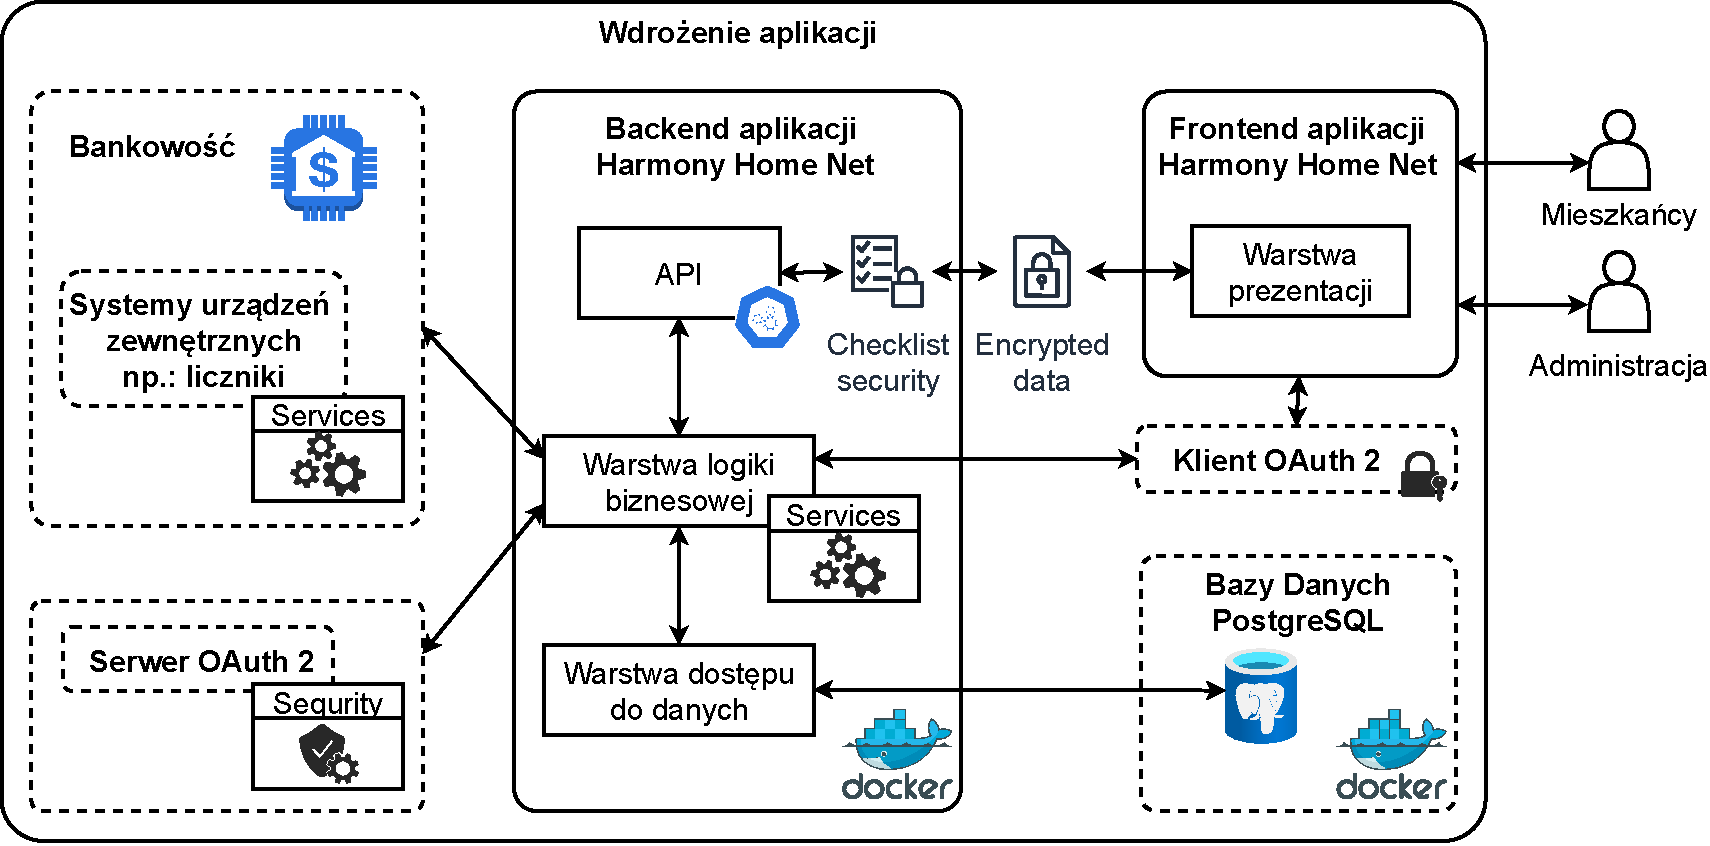
\includegraphics[width=1.1\linewidth]{Schematy/zarys_architektury}
		\caption{Schemat przestawiający zarys architektury systemu}
	\label{fig:zarys_architektury}
\end{figure}



\section{Wymagania aplikacji}
% TO DO: chyba na początek warto wyróżnić, w jakich rolach występować będą użytkownicy systemu i w ogóle - do czego ma służyć tworzona aplikacja

% Proszę zastanowić się, czy jednak nie dałoby się poniższego opisu jakoś rozwinąć (żeby nie był jedynie listą wyliczeniową). Czytelnik powinien zrozumieć, po co i dlaczego zdefiniowano poniższe wymagania. 

% Proszę zwrócić uwagę na "grupowanie" wymagań. Napisał Pan "Administrator zarządza lokalami ..." - ale trudno znaleźć wyjaśnienie, czym są te lokale i w ogóle - jaki to przypadek użycia (jaki jest kontekst, w jakim działać ma aplikacja).

Aplikacja eBOK (Elektroniczne Biuro Obsługi Klienta) jest narzędziem wspierającym zarządzanie wspólnotami mieszkaniowymi, które ma na celu poprawę komunikacji pomiędzy mieszkańcami a administracją oraz automatyzację procesów związanych z obsługą nieruchomości. Jednym z kluczowych aspektów aplikacji jest zarządzanie lokalami, które w systemie pełnią centralną rolę, gdyż każda funkcjonalność aplikacji – od zgłaszania usterek, przez płatności, po głosowania – jest związana z konkretnym lokalem.

Lokale, czyli nieruchomości (mieszkania, apartamenty, biura itp.), są podstawowym zasobem, który wymaga skutecznego zarządzania zarówno z perspektywy mieszkańca, jak i administratora. Dla mieszkańca lokal jest miejscem, do którego przypisane są należności finansowe, zgłoszenia techniczne czy dokumenty. Z perspektywy administratora, każdy lokal stanowi jednostkę, którą należy nadzorować pod kątem bieżących płatności, obsługi technicznej, jak również interakcji z właścicielami i najemcami. Dlatego zarządzanie lokalami/nieruchomościami w aplikacji eBOK jest jedną z kluczowych funkcji, zapewniającą przejrzystość oraz efektywność administracji.

\subsection{Przykłady użycia aplikacji}

Aplikacja eBOK oferuje różnorodne przypadki użycia, które ilustrują funkcjonalności dostępne dla różnych grup użytkowników. Głównym obszarem jej zastosowania jest zarządzanie relacją pomiędzy mieszkańcem a administratorem nieruchomości, w kontekście takich działań jak płatności, zgłoszenia usterek, dostęp do dokumentów czy udział w głosowaniach.

\begin{itemize} 

	\item \textbf{Mieszkańcy (właściciele i najemcy):} logując się do systemu, mają możliwość sprawdzenia należności za lokal, uregulowania opłat online oraz przeglądania historii rachunków. Mogą również zgłaszać usterki dotyczące lokalu (np. przeciek, awaria ogrzewania) i śledzić status zgłoszenia. Dodatkowo, mieszkaniecy ma dostęp do dokumentów związanych z jego lokalem, takich jak umowy, regulaminy czy faktury.
	
	\item \textbf{Administratorzy:} za pomocą panelu administracyjnego zarządzają zgłoszeniami technicznymi, przypisując je do wykonawców. Odpowiadają również za monitorowanie płatności związanych z każdym lokalem, a także za prowadzenie rejestru dokumentów i interakcje z mieszkańcami.
	
\end{itemize}

Każda z tych grup użytkowników ma dostęp do odpowiednich funkcji aplikacji, które spełniają jej potrzeby.

\subsection{Wymagania funkcjonalne}

Wymagania funkcjonalne aplikacji eBOK skupiają się na kluczowych obszarach działalności, które odpowiadają za sprawne funkcjonowanie wspólnoty mieszkaniowej.

\begin{enumerate}[label=\arabic*.] 

	\item \textbf{Zarządzanie kontem użytkownika i lokalami:} Użytkownicy muszą mieć możliwość tworzenia kont, zarządzania swoimi danymi osobowymi oraz przypisywania lokali do konta. Każdy mieszkaniec może przypisać do swojego konta lokal, którym zarządza lub w którym mieszka. W przypadku najmu, mieszkaniec może zarządzać umowami najmu oraz uprawnieniami innych użytkowników do korzystania z funkcji aplikacji dla tego lokalu.
	
	\item \textbf{Przegląd i płatność należności:} Mieszkańcy mogą przeglądać szczegółowe informacje na temat należności przypisanych do konkretnego lokalu. System umożliwia szybki dostęp do historii opłat oraz realizację płatności online. Powiadomienia o zaległościach związanych z danym lokalem przypominają mieszkańcom o konieczności uregulowania zobowiązań.

	\item \textbf{Zarządzanie zgłoszeniami technicznymi dla lokali:} Mieszkańcy mogą zgłaszać problemy techniczne dotyczące ich lokali, takie jak awarie czy uszkodzenia. Administrator przypisuje zgłoszenia do odpowiednich ekip serwisowych, monitorując postęp prac, co zwiększa transparentność działań i umożliwia szybką reakcję na zgłoszone problemy.
	
	\item \textbf{Zarządzanie dokumentami:} Lokale są również powiązane z dokumentami, takimi jak umowy najmu, protokoły przekazania, regulaminy czy faktury. Aplikacja pozwala na przechowywanie i udostępnianie tych dokumentów mieszkańcom oraz administratorom, eliminując konieczność używania tradycyjnych archiwów papierowych.
	
	\item \textbf{Głosowania mieszkańców:} W przypadku istotnych decyzji dotyczących zarządzania wspólnotą, administrator może organizować głosowania, w których mieszkańcy przypisani do poszczególnych lokali mogą wziąć udział. Dzięki aplikacji proces ten jest zautomatyzowany, a wyniki głosowań są dostępne w czasie rzeczywistym.
	
	\item \textbf{Powiadomienia i komunikacja:} System powiadomień informuje mieszkańców o ważnych wydarzeniach związanych z ich lokalem, takich jak zaległe płatności, zgłoszenia serwisowe czy nadchodzące głosowania. Personalizowane powiadomienia zapewniają, że mieszkańcy są na bieżąco z najważniejszymi informacjami dotyczącymi ich nieruchomości.

	\item \textbf{Panel administracyjny:} Administratorzy korzystają z zaawansowanego panelu, który pozwala im zarządzać wszystkimi lokalami, przypisanymi mieszkańcami oraz zgłoszeniami technicznymi. Panel umożliwia także monitorowanie płatności i generowanie raportów związanych z każdym lokalem, co jest kluczowe dla efektywnego zarządzania wspólnotą.
	
	\item \textbf{Integracja z zewnętrznymi systemami:} Aplikacja eBOK musi umożliwiać integrację z systemami takimi jak systemy pomiarowe liczników mediów (np. wodomierze, liczniki energii) oraz systemy płatności. Taka integracja usprawnia zarządzanie lokalami, umożliwiając automatyczne generowanie rachunków oraz synchronizację danych dotyczących zużycia mediów.
	
\end{enumerate}

\subsection{Wymagania niefunkcjonalne}

\begin{enumerate}[label=\arabic*.] 

	\item \textbf{Skalowalność:} System musi być na tyle elastyczny, aby mógł obsługiwać zarówno małe wspólnoty mieszkaniowe, jak i większe spółdzielnie, z możliwością zarządzania setkami lub tysiącami lokali.

	\item \textbf{Dostępność:} Aplikacja musi działać 24/7 i być dostępna z każdego urządzenia podłączonego do Internetu, co zapewnia mieszkańcom możliwość zarządzania ich lokalami w dowolnym momencie.

	\item \textbf{Bezpieczeństwo:} Ważnym aspektem jest ochrona danych użytkowników oraz dokumentów związanych z lokalami. System musi zapewniać szyfrowanie danych, uwierzytelnianie dwuskładnikowe oraz ochronę przed zagrożeniami takimi jak ataki SQL Injection czy XSS.

	\item \textbf{Wydajność:} Aplikacja powinna działać płynnie, nawet w przypadku dużego obciążenia, co jest szczególnie istotne przy przetwarzaniu dużych ilości danych związanych z lokalami i płatnościami.

	\item \textbf{Intuicyjność interfejsu:} Interfejs aplikacji powinien być prosty i intuicyjny, zarówno dla mieszkańców, jak i administratorów. Właściciele lokali powinni mieć możliwość łatwego zarządzania danymi swojego lokalu, zgłaszania problemów i przeglądania dokumentów bez potrzeby przechodzenia przez skomplikowane procedury.

\end{enumerate}
